\documentclass[]{article}

\usepackage{cite} % For citations
\usepackage[backref]{hyperref} % For hyperlinks and references
\usepackage{amsmath} % For math expressions
\usepackage{graphicx} % For including graphics
\usepackage{fancyhdr} % For custom headers and footers
\usepackage{subcaption} % For subfigures
\usepackage{float} % For better figure placement control

\title{\textbf{Computer Vision homework 4}}
\author{Pan Changxun 2024011323}
\date{May 2025}

\topmargin=-0.45in      %
\evensidemargin=0in     %
\oddsidemargin=0in      %
\textwidth=6.5in   
\textheight=9.0in       %
\headsep=0.25in 

\pagestyle{fancy}
\fancyhf{} % Clear all header and footer fields
\fancyhead[L]{Pan Changxun} % Left header
\fancyhead[C]{Computer Vision homework 4} % Center header
\fancyhead[R]{May 2025} % Right header
%\fancyfoot[L]{\leftmark} % Left footer
\fancyfoot[C]{\thepage} % Center footer
%\fancyfoot[R]{} % Right footer

\begin{document}
\maketitle

\section{Introduction}
This report documents the implementation of the DeepLabV3+ model for semantic segmentation on the Cityscapes dataset. The goal is to achieve high accuracy in segmenting urban scenes into 19 different classes, such as road, car, pedestrian, etc. The report covers the model architecture, training strategy, and evaluation metrics.

The codes for this project are available in the GitHub repository: \url{https://github.com/CXP-2024/CV-hw/tree/main/CV-hw4}.
A detailed description can be obtained from the README file in the repository. 

I build my own version of the deeplabv3plus model base on the original implementation, which is also described in the MODEL.md file in the repository or see it in \ref{sec:Models}. For detailed evaluation, see the EVALUATION.md file in the repository. A brief summary is provided in \ref{sec:Evaluation}.

Some tricks I used in the training process include:
\begin{itemize}
		\item Implemented a 5-fold cross-validation strategy to improve model robustness and reduce overfitting.
		\item Employed a combination of label smoothing cross-entropy loss and Dice loss to enhance segmentation performance. See \ref{sec:Loss_Function} for details.
		\item Utilized data augmentation techniques to increase the diversity of training samples and improve generalization. See \ref{sec:Data_Augmentation} for brief details and the EVALUATION.md file for more details.
		\item Implemented a cosine learning rate scheduler for better convergence during training. 
		\item Experimented with different model aggregation strategies to optimize final performance. See \ref{sec:Model_Aggregation} for details.
\end{itemize}

Finally, I use the DeepLabV3+ model to achieve a mean Intersection over Union (mIoU) of 61.9\% (Figure~\ref{fig:train_metrics_10_149}, \ref{fig:per_class_iou}) on the official validation set. All the figures see in \ref{sec:Figures}.


\section{Experiments and Results}\label{sec:Experiments}
\subsection{Initial Training without Cross-Validation}
I initially conducted experiments without cross-validation to establish a baseline. However, I observed that the model quickly began to overfit, with the loss no longer decreasing after a certain point. Despite this limitation, the model achieved a mean Intersection over Union (mIoU) of approximately 51\%. The training curve is shown in Figure~\ref{fig:no_cross_val_10_30}.

To address the overfitting issue, I implemented a 5-fold cross-validation approach by \textbf{splitting the official training set into five subsets}. The combined loss with weighting between label smoothed cross-entropy and Dice loss (0.6:0.4) proved most effective during this phase. This significantly improved performance, with the mIoU reaching approximately 54\% by the end of training. Figure~\ref{fig:cross_val_10_30_val} compares mIoU across all folds on the official validation set.

\subsection{Training Results for Epochs 30-50}
During the second training phase (epochs 30-50), I observed a slight decrease in overall performance. However, the averaged model still maintained a respectable mIoU of 54\%, indicating the robustness of the model averaging approach but seemingly no improvement. The model aggregation show in Figure~\ref{fig:3model_comparison_30_50} highlights the performance differences between the three aggregation strategies. The best performing model from this phase was then used as the pre-trained model for the next training iteration.


\subsection{Training Results for Epochs 50-70}
Encouragingly, after I apply data augmentation techniques (The level I choose "standard" first), performance improved during the third training phase (epochs 50-70), with the best model achieving an mIoU of 56\%. This improvement suggests that the learning rate adjustment strategy and continued training were effective in refining the model parameters. The results of this training phase are presented in Figures~\ref{fig:cross_val_50_70_val}, showing the detailed performance metrics across different folds.

\subsection{Training Results for Epochs 70-150}
For the later training phase, I choose "advanced" data augmentation, which includes more aggressive transformations. And start to use the cosine learning rate strategy. 



\subsection{Final Optimization and Results}\label{sec:Final_Optimization}
Given the performance plateau and the significant variance, I decided to conclude the training at this point. (I also tried to use the warmup learning rate strategy, but it did not yield better results. I find when the learning rate is reset after the period, the optimization process is not as effective as the cosine learning rate strategy.(not stable))

The final test results are presented in Figures~\ref{fig:per_class_iou}, \ref{fig:confusion_matrix}, and \ref{fig:class_weight_vs_iou}, with detailed visualizations available in the directory \texttt{outputs/deeplabv3plus\_test\_results}. Figure~\ref{fig:per_class_iou} shows the per-class IoU scores, Figure~\ref{fig:confusion_matrix} presents the confusion matrix for segmentation results, and Figure~\ref{fig:class_weight_vs_iou} illustrates the relationship between class weights and IoU scores. Figure~\ref{fig:3model_comparison} compares the performance of the three model aggregation approaches.


\section{Models}\label{sec:Models}
I first tried to use the UNet model, but it did not perform well for this segmentation task. I then implemented the DeepLabV3 model and further improved it to DeepLabV3+. The DeepLabV3+ architecture consists of the following key components:

\begin{itemize}
    \item A backbone network using ResNet with atrous convolutions
    \item Atrous Spatial Pyramid Pooling (ASPP) to capture multi-scale context
    \item A decoder module that refines the segmentation results
    \item Skip connections that combine low-level features with high-level features
\end{itemize}

This architecture is particularly effective for semantic segmentation tasks as it captures both detailed spatial information and broad contextual information.

\subsection{Model Architecture Details}
The DeepLabV3+ model I implemented consists of several carefully designed components:

\subsubsection{ResNet Backbone}
I implemented a custom ResNet backbone with atrous (dilated) convolutions:
\begin{itemize}
    \item Initial layer: 7×7 convolution with stride 2, followed by batch normalization, ReLU, and max pooling
    \item Layer 1: 3 ResNet blocks with 64 channels
    \item Layer 2: 4 ResNet blocks with 128 channels, stride 2
    \item Layer 3: 6 ResNet blocks with 256 channels, dilation rate 2
    \item Layer 4: 3 ResNet blocks with 512 channels, dilation rate 4
\end{itemize}

Each ResNet block consists of two 3×3 convolutional layers with batch normalization and ReLU, along with a residual connection. The increasing dilation rates in deeper layers ensure a larger receptive field without decreasing spatial resolution.

\subsubsection{ASPP Module}
The Atrous Spatial Pyramid Pooling module consists of:
\begin{itemize}
    \item One 1×1 convolution
    \item Three 3×3 atrous convolutions with dilation rates of 12, 24, and 36
    \item A global average pooling branch followed by a 1×1 convolution
\end{itemize}

These five branches are concatenated and fed through a 1×1 convolution with 256 output channels, followed by batch normalization, ReLU, and a dropout layer (rate=0.5) to obtain the final ASPP features.

\subsubsection{Decoder Module}
The decoder integrates the semantically rich features from the ASPP module with spatially detailed low-level features from earlier layers:
\begin{itemize}
    \item Low-level features from the first ResNet layer are processed by a 1×1 convolution to reduce channels to 48
    \item ASPP features are upsampled to match the spatial dimensions of the low-level features
    \item Both feature maps are concatenated and processed by two 3×3 convolutions
    \item The result is then upsampled to input resolution and fed to a final classifier
\end{itemize}

\subsubsection{Final Classification Layer}
A simple 1×1 convolution transforms the decoder output into class logits with 19 channels (one for each class in the Cityscapes dataset).

\subsubsection{Weight Initialization}
All convolutional layers use Kaiming initialization to ensure proper gradient flow during training, while batch normalization layers are initialized with weight=1 and bias=0.



\subsection{Model Input and Evaluation Resolution}
To balance performance and computational efficiency, all training and evaluation were conducted at a consistent resolution of 512×1024 pixels. The original Cityscapes images (1024×2048) were resized to this working resolution during both training and testing phases.

This resolution choice was explicitly defined in the \texttt{config.yaml} file:
\begin{verbatim}
data:
  image_size: [512, 1024]  # height, width
\end{verbatim}

Both input images and ground truth labels were resized to this resolution. During inference, the model predictions remain at 512×1024 resolution rather than being upscaled back to the original 1024×2048 resolution. This approach ensures consistency between training and evaluation conditions, while significantly reducing memory requirements and computational load.

The model architecture was designed to handle this specific resolution, with the encoder progressively reducing spatial dimensions and the decoder carefully upsampling features back to the input dimensions. The final interpolation layer in the DeepLabV3+ model upsamples the features to match the input resolution of 512×1024:

\begin{verbatim}
# Upscale to input resolution
x = F.interpolate(x, size=input_shape, mode='bilinear', align_corners=False)
\end{verbatim}

This consistent handling of resolution across both training and evaluation phases ensures fair comparisons and reliable performance metrics.

\section{Finial Evaluation Resolution Strategy}\label{sec:Evaluation}
For the final evaluation on the validation set, I implemented two distinct approaches to assess the model's performance under different resolution conditions:

\subsection{Fixed Working Resolution Evaluation}
In the first approach (implemented in \texttt{test\_deeplabv3plus.py}), both input images and evaluation metrics were processed at the consistent working resolution of 512×1024 pixels. This approach maintains perfect alignment with the training conditions, allowing for a direct assessment of the model's performance without introducing resolution-related variables.

\subsection{Original Resolution Evaluation}
The second approach (implemented in \textbf{\texttt{test\_deeplabv3plus\_origin\_resolution.py})} was designed to evaluate the model under real-world deployment conditions where output is needed at the original high resolution. In this pipeline:
\begin{itemize}
	\item Input images are downsampled from 1024×2048 to 512×1024 for model inference
	\item The resulting predictions are then upsampled back to the original 1024×2048 resolution
	\item Evaluation metrics (including mIoU) are calculated at the full 1024×2048 resolution
\end{itemize}
This approach provides insights into how the model's predictions translate to full-resolution applications. While this method typically yields slightly lower mIoU scores compared to the fixed resolution evaluation (approximately 0.06\% decrease), it provides a more realistic assessment of the model's practical performance on high-resolution imagery. The difference in performance highlights the challenges of resolution changes in semantic segmentation tasks.

\section{Loss Function Design}\label{sec:Loss_Function}

For loss calculation, I implemented a comprehensive loss function strategy to address the challenges of semantic segmentation. Initially, I used standard cross-entropy loss during the first training phase. For later training stages, I developed a more sophisticated combined loss approach found in \texttt{utils/losses.py}.

My loss function implementation consists of three main components:

\subsection{Label Smoothing Cross Entropy Loss}
To reduce overfitting and improve model generalization, I implemented label smoothing for the cross-entropy loss. Rather than using hard targets (1 for correct class, 0 for others), label smoothing assigns a value slightly less than 1 to the correct class and small non-zero values to other classes:

\begin{itemize}
    \item For the correct class: target = $1 - \text{smoothing}$
    \item For other classes: target = $\text{smoothing} / \text{num\_classes}$
\end{itemize}

This technique helps prevent the model from becoming overconfident and improves its ability to generalize. I used a smoothing factor of 0.1, which provided a good balance between confidence and generalization.

\subsection{Dice Loss}
To directly optimize for the intersection over union metric, I implemented Dice loss, which is particularly effective for segmentation tasks with class imbalance. The Dice coefficient measures the overlap between predicted and ground truth segmentations:

\begin{equation}
\text{Dice} = \frac{2 \times \text{intersection} + \text{smooth}}{\text{union} + \text{smooth}}
\end{equation}

Where:
\begin{itemize}
    \item intersection = sum of element-wise multiplication of predictions and targets
    \item union = sum of predictions + sum of targets
    \item smooth = a small constant (1.0) to prevent division by zero
\end{itemize}

The Dice loss is calculated as $1 - \text{Dice}$, so minimizing this loss maximizes the Dice coefficient.

\subsection{Combined Loss Function}
To leverage the benefits of both approaches, I created a combined loss function that is a weighted sum of label smoothing cross-entropy and Dice loss:

\begin{equation}
\text{Loss} = \alpha \times \text{CrossEntropyLoss} + (1-\alpha) \times \text{DiceLoss}
\end{equation}

Where $\alpha = 0.6$ gives equal weight to both loss components.

This combined approach addresses multiple challenges:
\begin{itemize}
    \item Cross-entropy provides stable gradients and good convergence properties
    \item Label smoothing prevents overconfidence and improves generalization
    \item Dice loss directly optimizes for overlap metrics (similar to IoU)
    \item The combination helps balance between pixel-wise accuracy and region-based segmentation quality
\end{itemize}

Additionally, all loss functions properly handle ignored pixels (labeled with 255) and support class weights to address class imbalance issues.


\section{Model Aggregation}\label{sec:Model_Aggregation}
After training all folds, I evaluated three model aggregation approaches:
\begin{enumerate}
    \item The best mIoU model from all folds
    \item The average of parameters from the best models across all folds
    \item The average of parameters from the top 3 best mIoU models across all folds
\end{enumerate}

The best performing model from these three approaches was then used as the pre-trained model for the next 20-epoch training iteration. Since the initial training was for 10 epochs, subsequent training stages began at epochs 10, 30, 50, etc.

The results for the first cross-validation stage (epochs 10-30) are shown in Figure~\ref{fig:cross_val_10_30_val}. 
\section{Data augmentation}\label{sec:Data_Augmentation}
To improve model generalization, I implemented a three-level data augmentation framework for the Cityscapes dataset:

\begin{enumerate}
    \item \textbf{None}: No augmentation, only image resizing to target dimensions
    \item \textbf{Standard}: A set of basic augmentations including horizontal flipping (50\% probability), Gaussian blur (30\%), gamma adjustment (25\%), random upscaling (50\%), random cropping (40\%), and color jittering (50\%)
    \item \textbf{Advanced}: All standard augmentations plus more aggressive transformations like color channel swapping (10\%), grayscale conversion (10\%), sharpening (10\%), color balance adjustment (10\%), enhanced color jittering (15\%), noise addition (10\%), modified elastic transformation (10\%), and color-based image mixup (5\%)
\end{enumerate}

The augmentation level could be specified in the configuration file or overridden via command-line arguments. For cross-validation, the data module ensured that:
\begin{itemize}
    \item Training folds received the specified augmentation level
    \item Validation folds always used 'none' augmentation to maintain evaluation consistency
    \item Each fold received independent dataset copies with appropriate transform settings
\end{itemize}

All transformations were carefully designed to preserve semantic integrity by avoiding black border artifacts, using reflection padding instead of constant black values, and preventing confusing scenes through selective application of transforms.



\section{Acknowledgements}
I would like to acknowledge the authors of the DeepLabV3+ architecture, whose work provided the foundation for this implementation. I also utilized GitHub Copilot as a programming assistant to help streamline code development and debugging.
\section{Figures}\label{sec:Figures}

\begin{figure}[htbp]
		\centering
		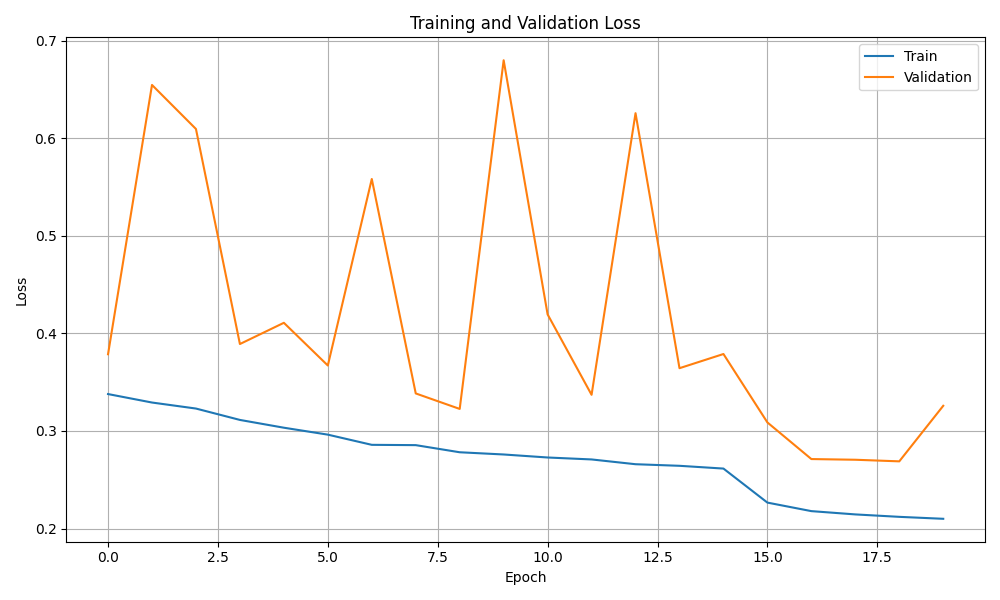
\includegraphics[width=0.8\textwidth]{no_cross_val_10_30.png}
		\caption{Training curve for epochs 10 to 30 without cross-validation, showing signs of overfitting}
		\label{fig:no_cross_val_10_30}
\end{figure}

\begin{figure}[htbp]
		\centering
		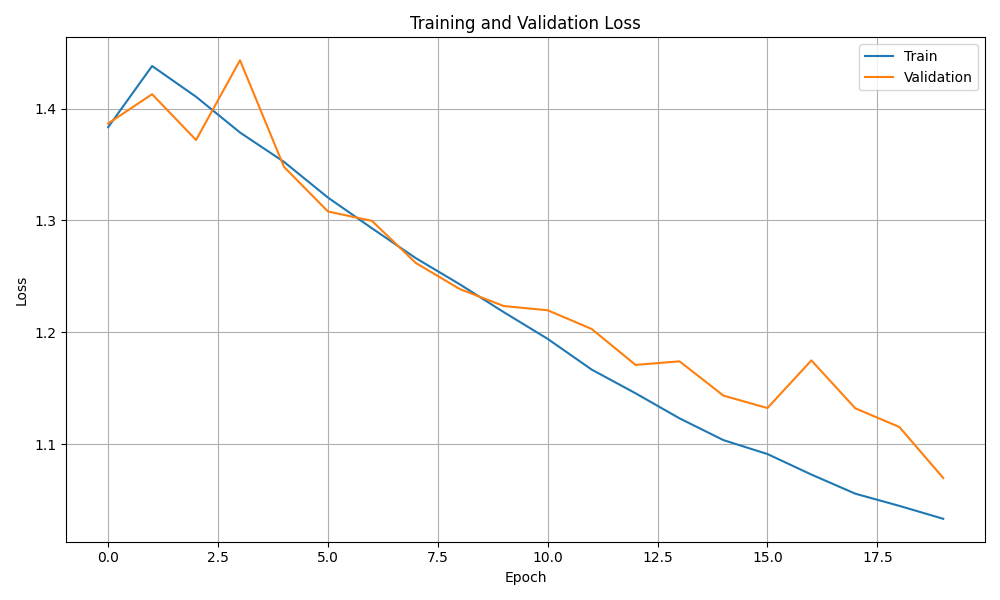
\includegraphics[width=0.8\textwidth]{cross_10_30.png}
		\caption{Training curve for epochs 10 to 30 with cross-validation, showing improved generalization}
		\label{fig:cross_val_10_30}
\end{figure}

%training_metrics_epoch_10_to_69
\begin{figure}[htbp]
		\centering
		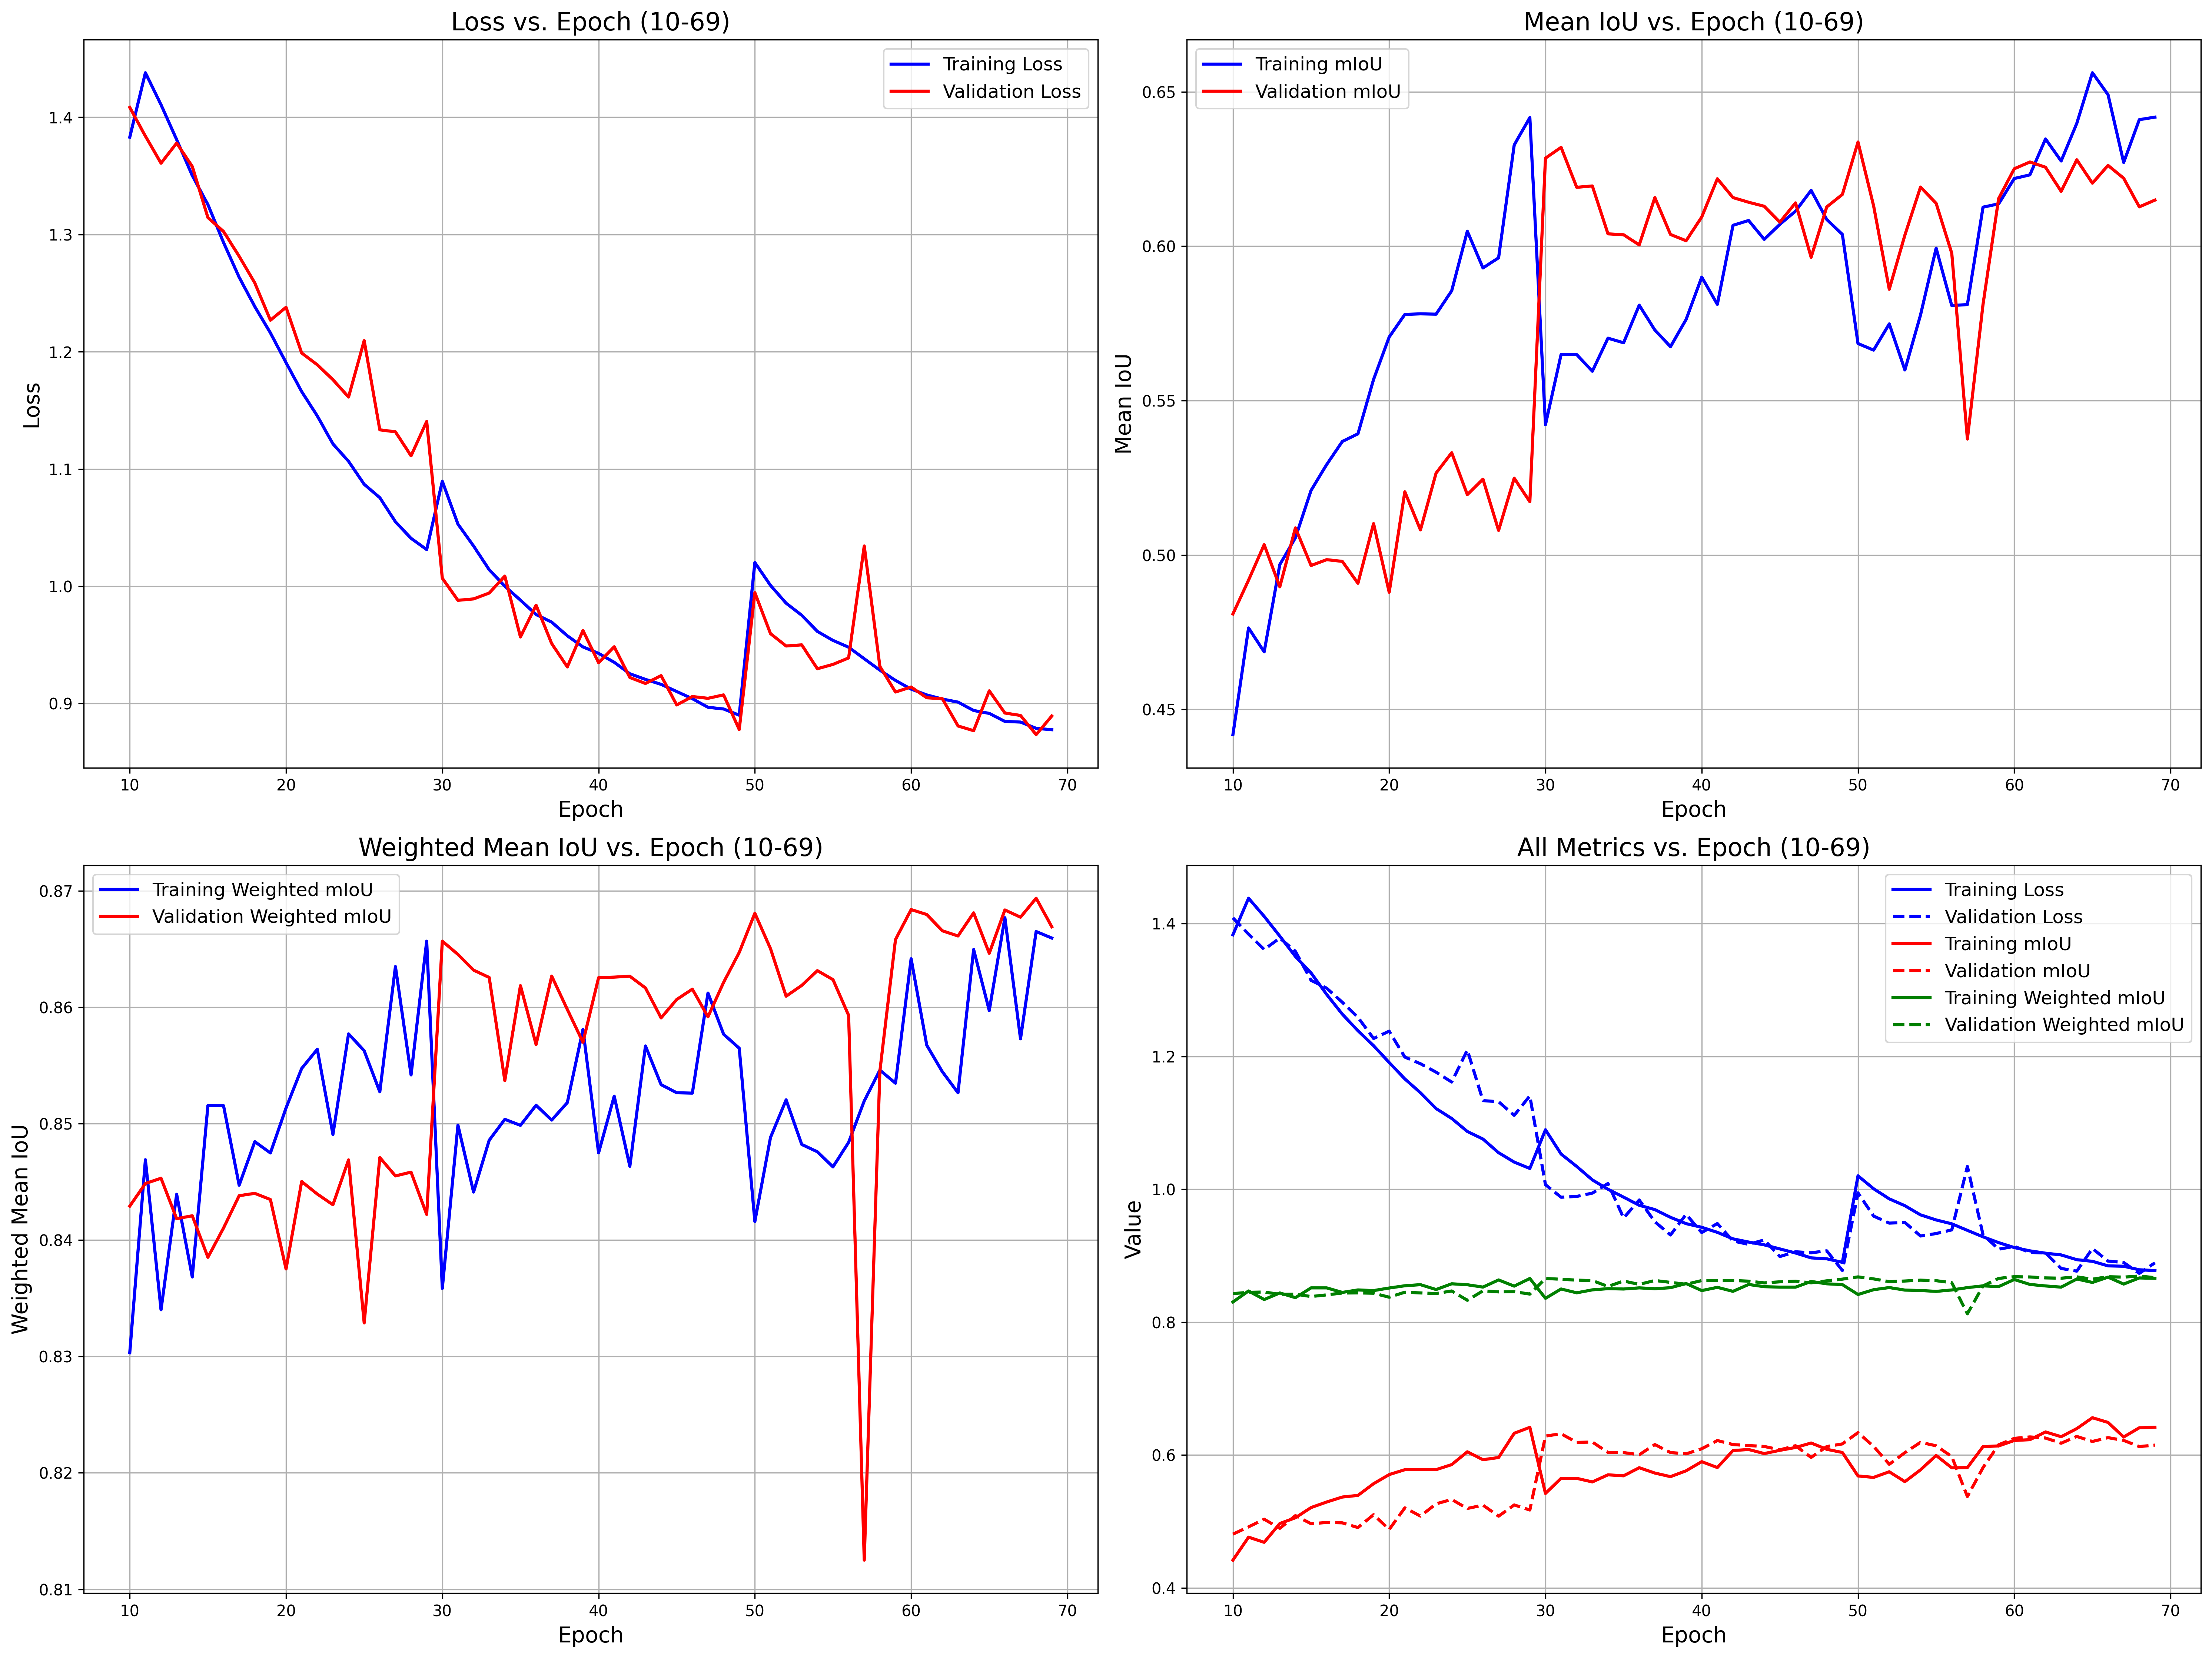
\includegraphics[width=1.0\textwidth]{outputs/deeplabv3plus_test_results/early_training_epochs_10_to_69.png}
		\caption{Training metrics for epochs 10-69 for fold 1, showing performance patterns throughout consecutive training intervals with cosine learning rate scheduling and model aggregation applied after each 20-epoch segment}
		\label{fig:train_metrics_10_69}
\end{figure}

\begin{figure}[htbp]
    \centering
    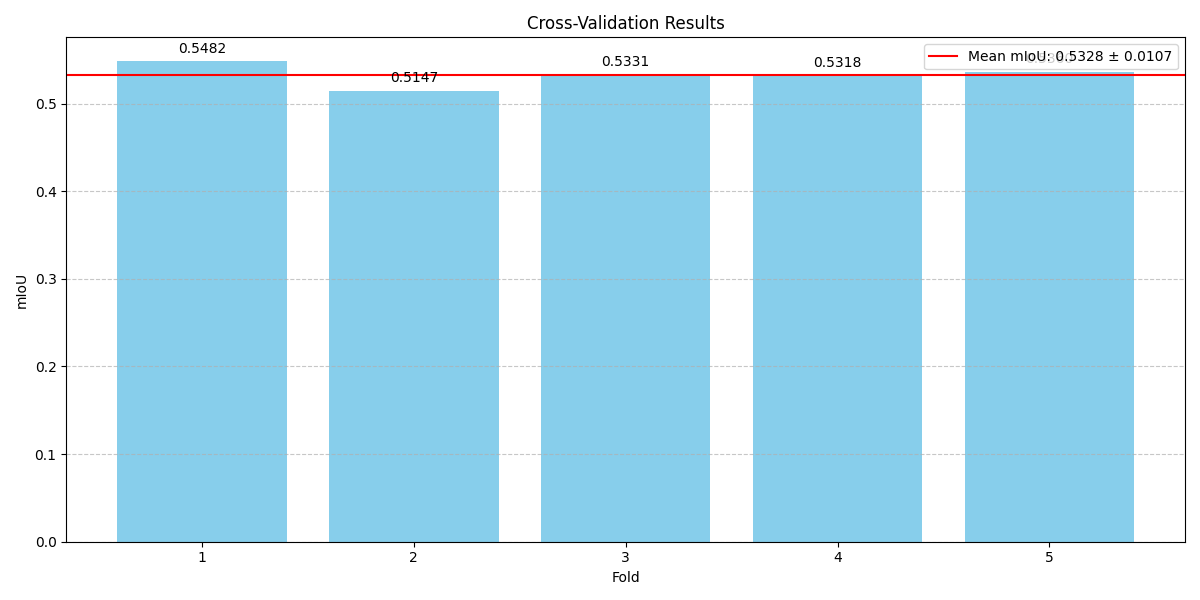
\includegraphics[width=0.8\textwidth]{folds_10_30.png}
    \caption{mIoU comparison across all folds on the official validation set, epochs 10-30}
    \label{fig:cross_val_10_30_val}
\end{figure}


\begin{figure}[htbp]
    \centering
    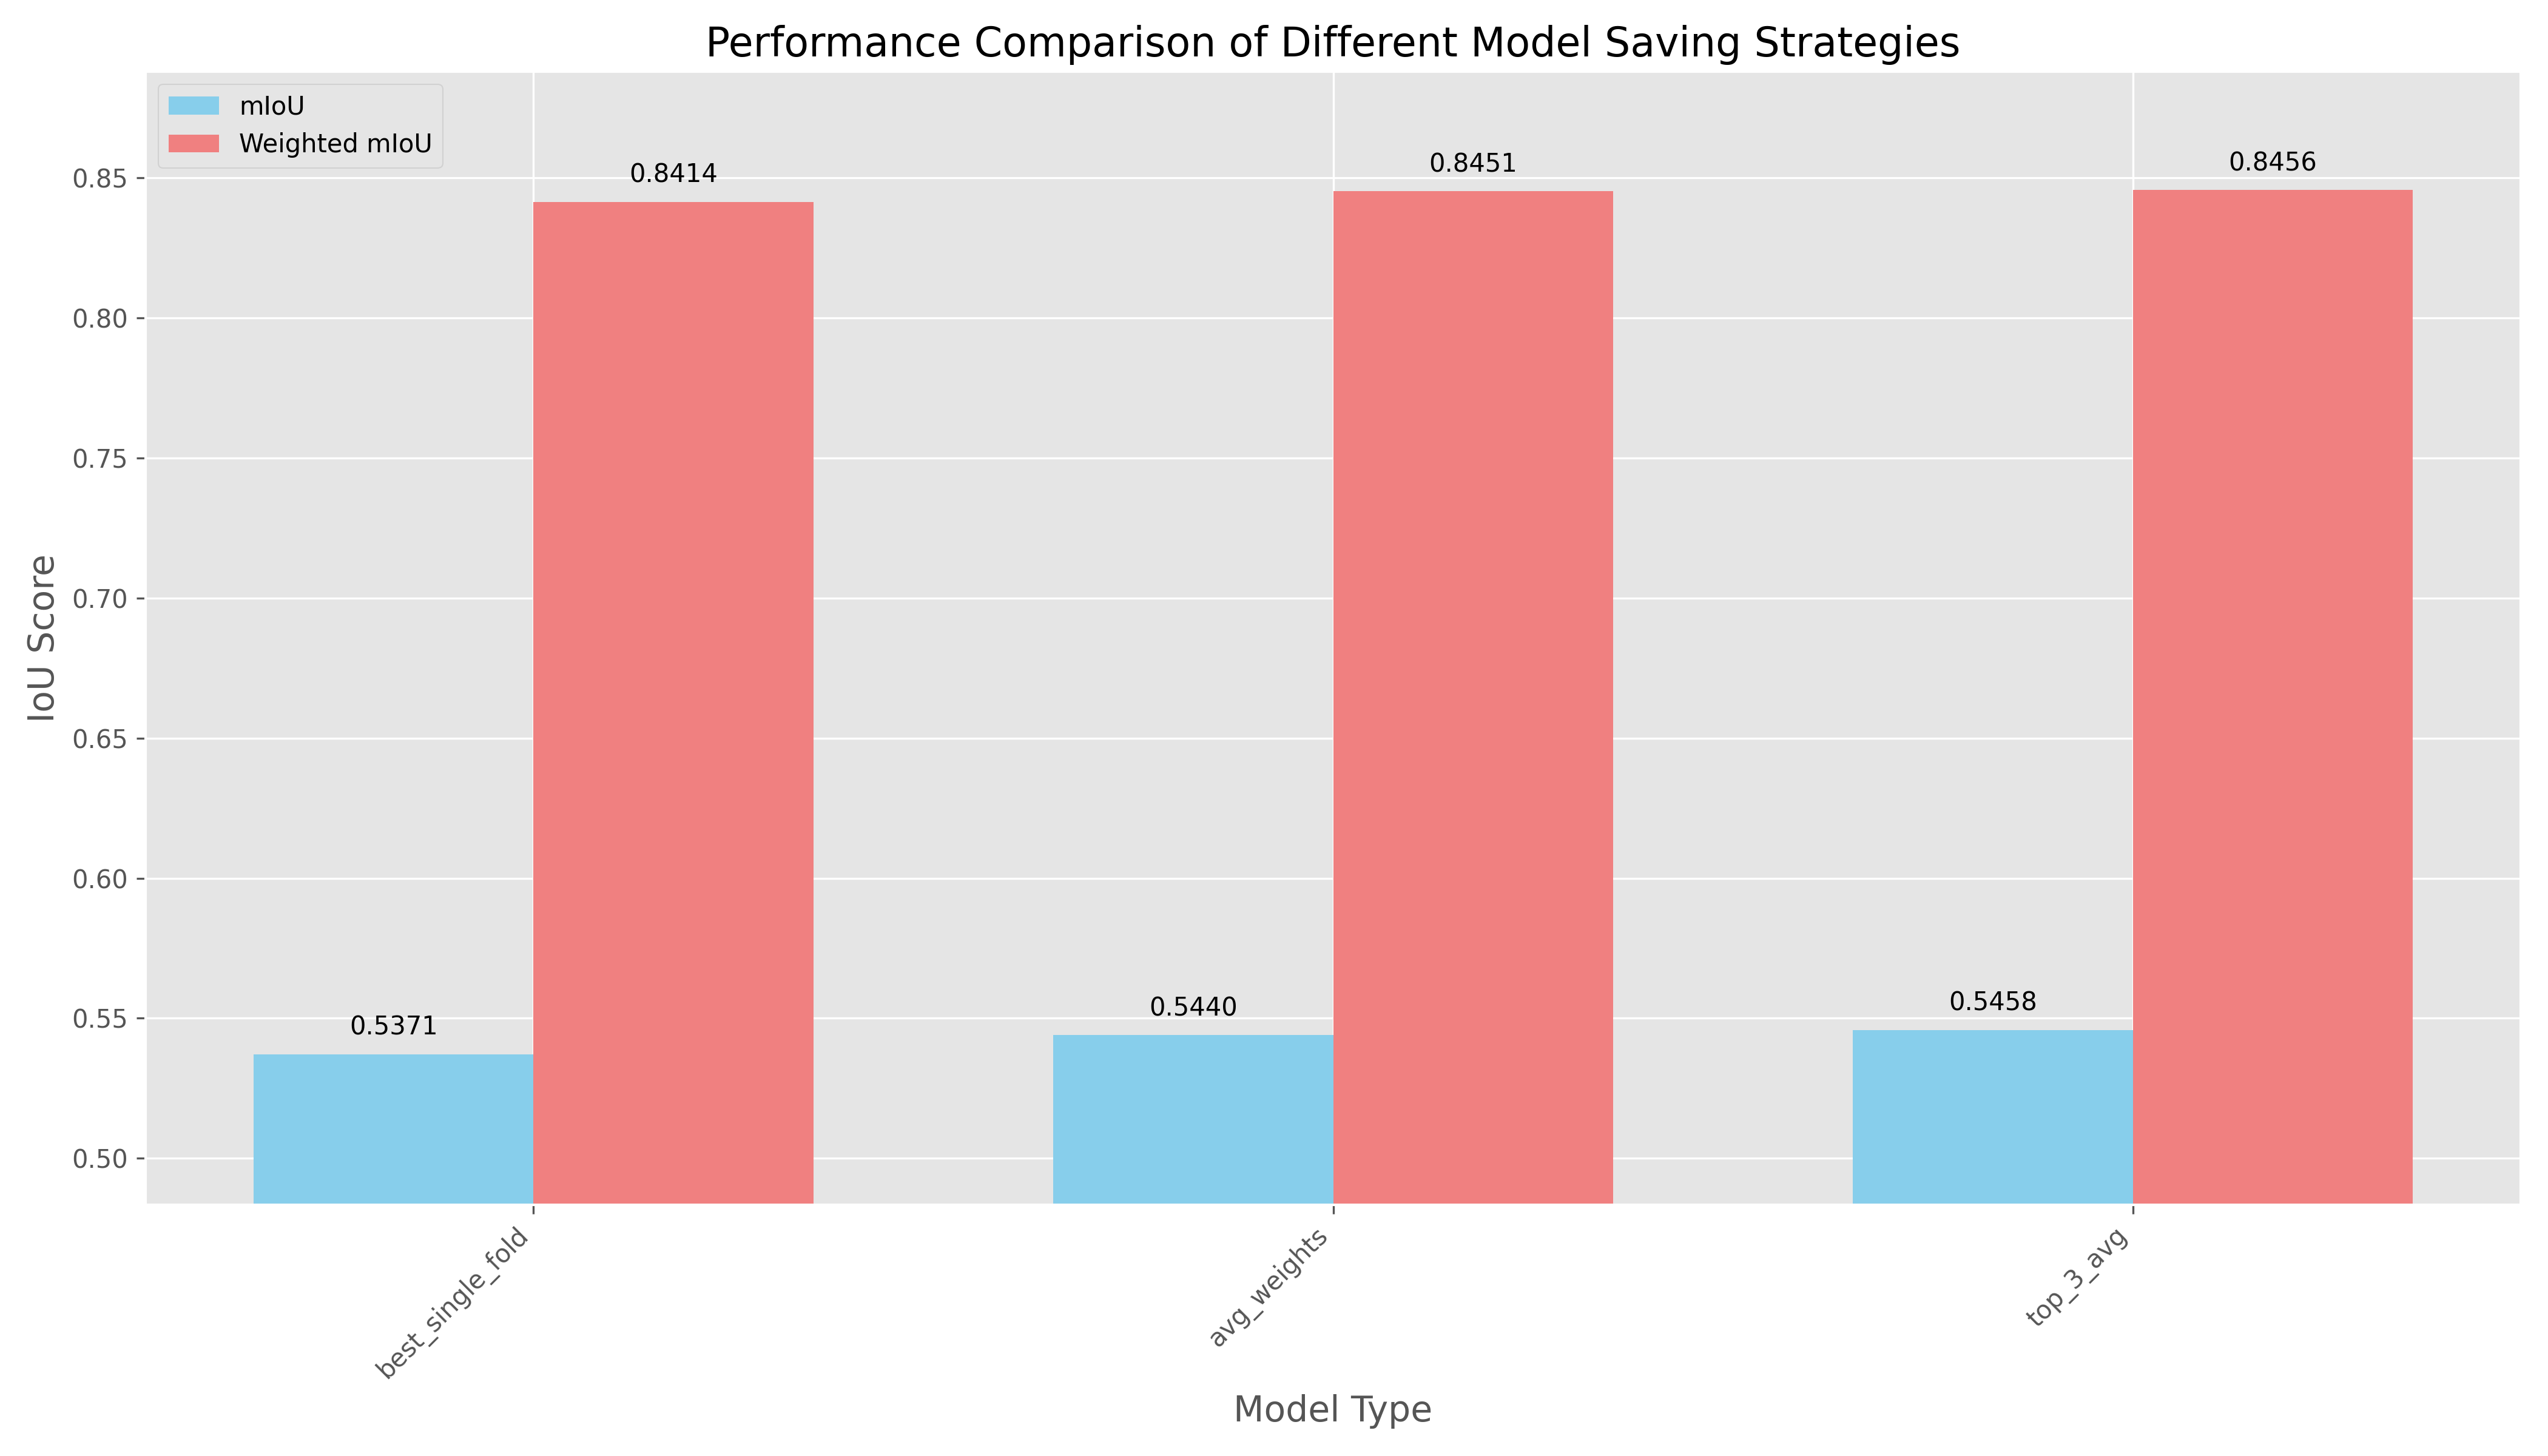
\includegraphics[width=0.8\textwidth]{3model_comparison_30_50.png}
    \caption{Comparison of the three model aggregation approaches for epochs 30-50, highlighting their performance differences}
    \label{fig:3model_comparison_30_50}
\end{figure}



\begin{figure}[htbp]
    \centering
    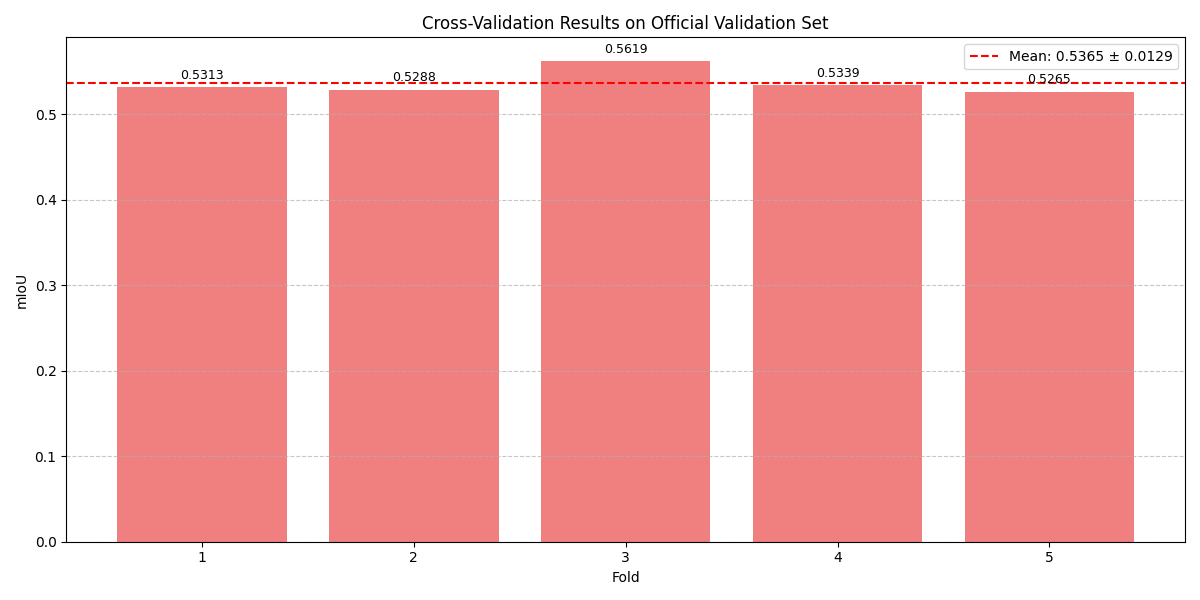
\includegraphics[width=0.8\textwidth]{folds_50_70.png}
    \caption{mIoU comparison across all folds on the official validation set, epochs 50-70}
    \label{fig:cross_val_50_70_val}
\end{figure}

%train_metrics_70_150.png
\begin{figure}[htbp]
    \centering
    \includegraphics[width=1.0\textwidth]{outputs/deeplabv3plus_test_results/training_metrics_epoch_70_to_149.png}
		\caption{Training metrics for epochs 70-150 for fold 1, showing performance patterns throughout consecutive training intervals with cosine learning rate scheduling and model aggregation applied after each 20-epoch segment}
    \label{fig:train_metrics_70_150}
\end{figure}

%folds 70_90.png
\begin{figure}[htbp]
		\centering
		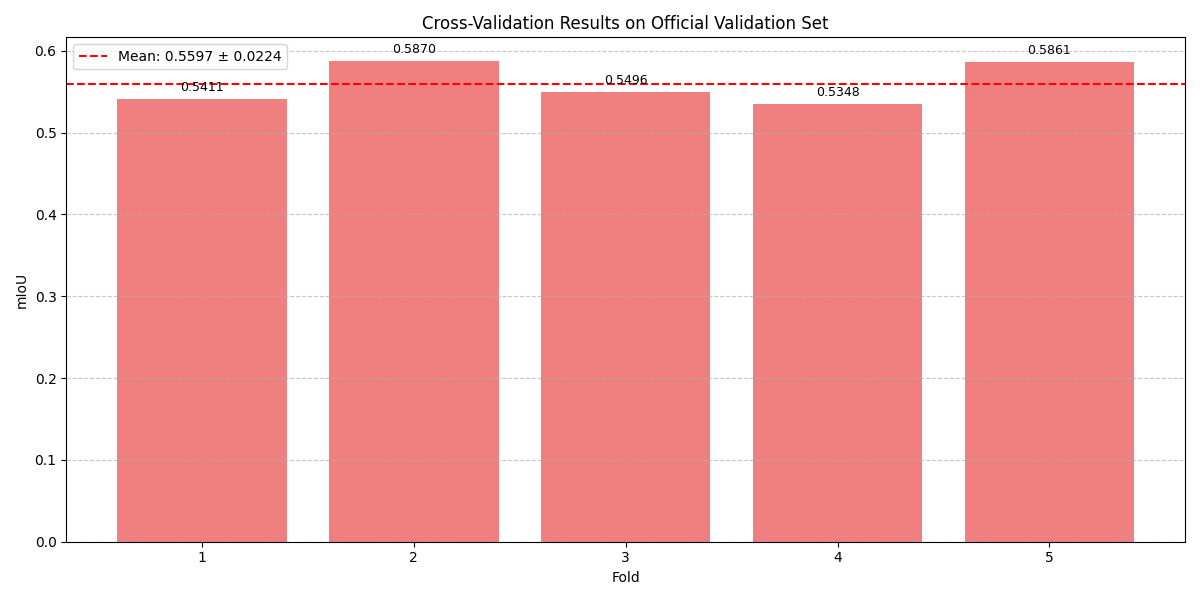
\includegraphics[width=0.8\textwidth]{folds_70_90.png}
		\caption{mIoU comparison across all folds on the official validation set, epochs 70-90}
		\label{fig:cross_val_70_90_val}
\end{figure}

%folds 90_110.png
\begin{figure}[htbp]
		\centering
		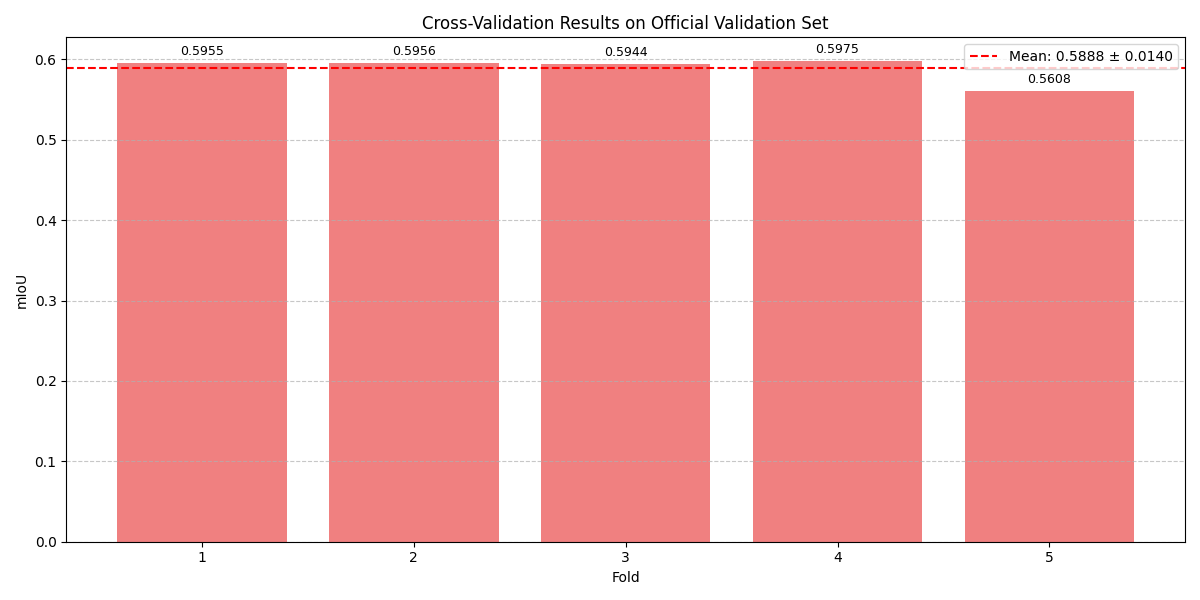
\includegraphics[width=0.8\textwidth]{folds_90_110.png}
		\caption{mIoU comparison across all folds on the official validation set, epochs 90-110}
		\label{fig:cross_val_90_110_val}
\end{figure}

%folds 110_130.png
\begin{figure}[htbp]
		\centering
		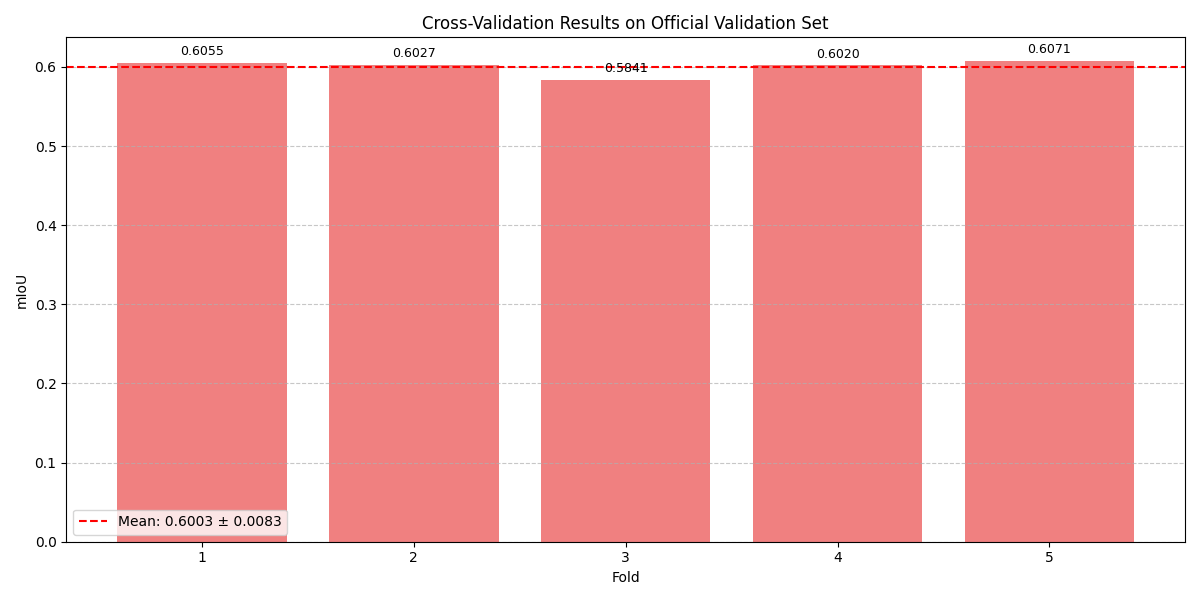
\includegraphics[width=0.8\textwidth]{folds_110_130.png}
		\caption{mIoU comparison across all folds on the official validation set, epochs 110-130}
		\label{fig:cross_val_110_130_val}
\end{figure}

%folds 130_150.png
\begin{figure}[htbp]
		\centering
		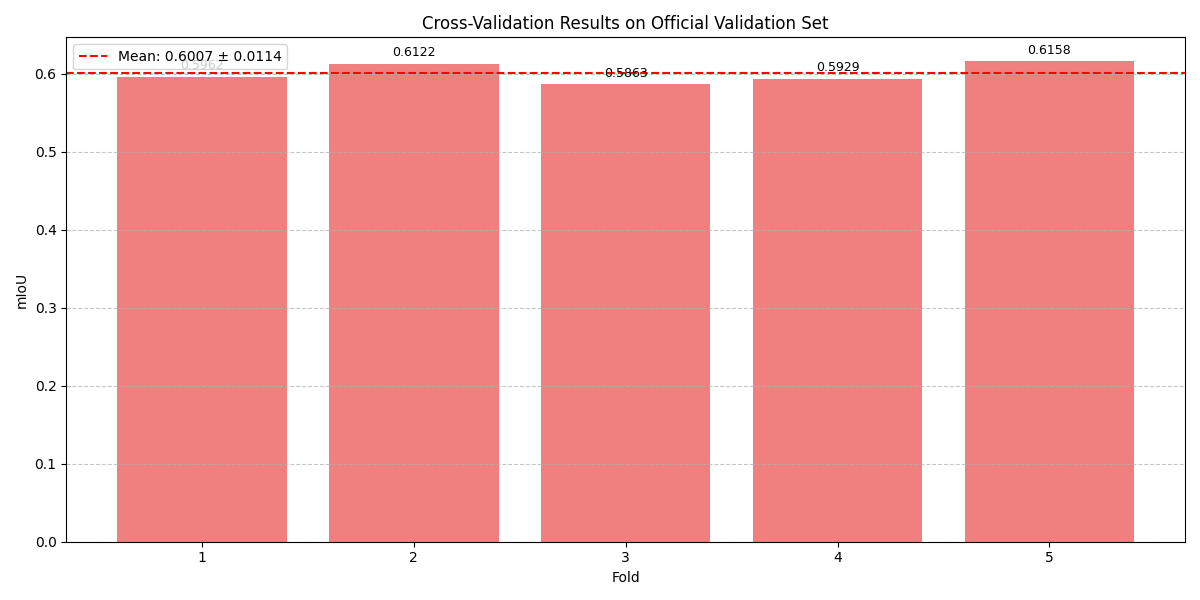
\includegraphics[width=0.8\textwidth]{folds_130_150.png}
		\caption{mIoU comparison across all folds on the official validation set, epochs 130-150}
		\label{fig:cross_val_130_150_val}
\end{figure}

%training_metrics_epoch_10_to_149.png
\begin{figure}[htbp]
		\centering
		\includegraphics[width=1.0\textwidth]{outputs/deeplabv3plus_test_results/training_metrics_epoch_10_to_149.png}
		\caption{Training metrics for epochs 10-149 for fold 1, showing performance patterns throughout consecutive training intervals with cosine learning rate scheduling and model aggregation applied after each 20-epoch segment}
		\label{fig:train_metrics_10_149}
\end{figure}

\begin{figure}[htbp]
    \centering
    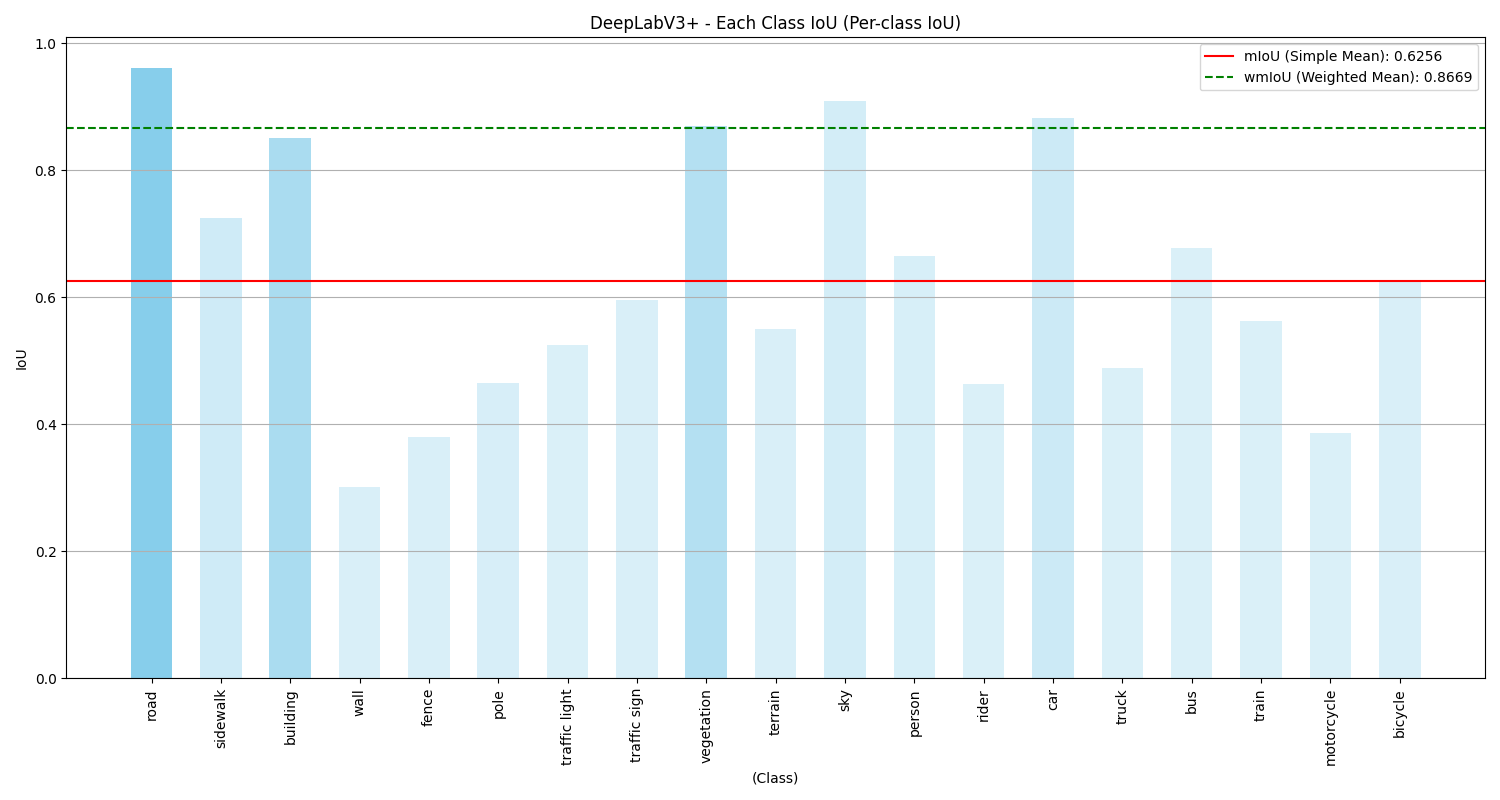
\includegraphics[width=0.8\textwidth]{outputs/deeplabv3plus_test_results/per_class_iou.png}
    \caption{Per-class IoU scores for the final model, showing the model's performance across different semantic categories}
    \label{fig:per_class_iou}
\end{figure}

\begin{figure}[htbp]
    \centering
    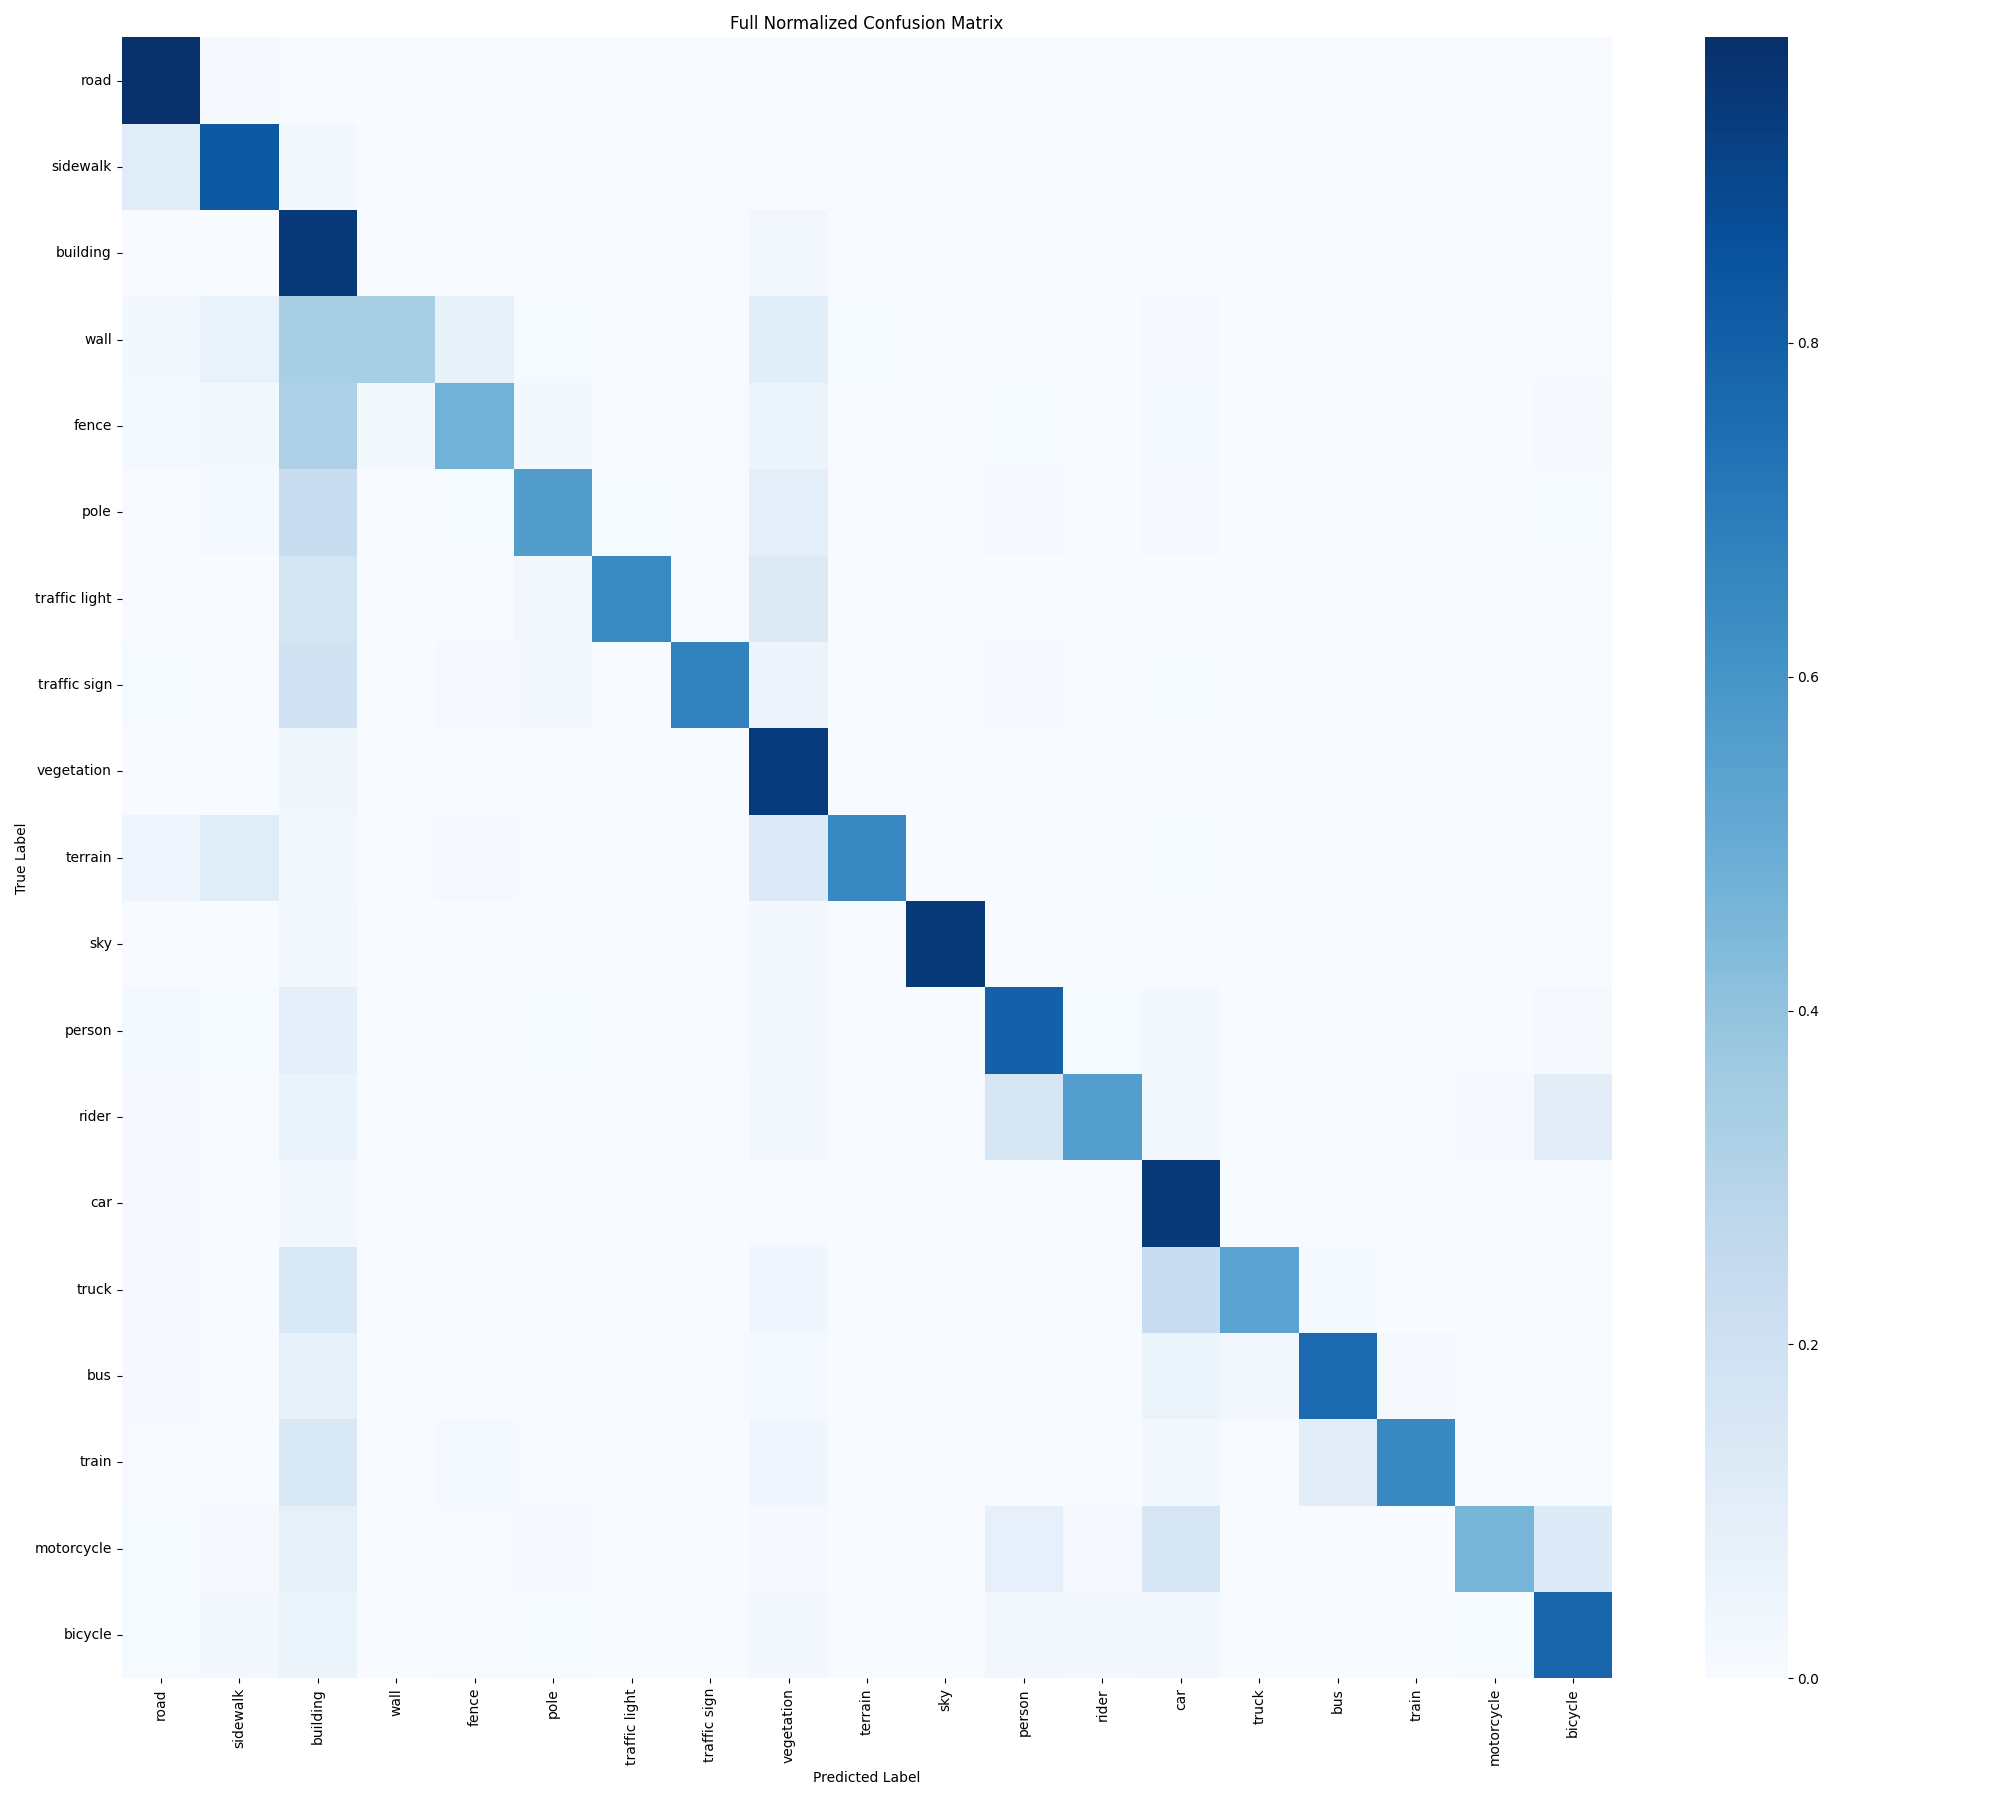
\includegraphics[width=0.8\textwidth]{outputs/deeplabv3plus_test_results/full_confusion_matrix.png}
    \caption{Confusion matrix for the segmentation results, illustrating the distribution of predicted classes versus ground truth}
    \label{fig:confusion_matrix}
\end{figure}

\begin{figure}[htbp]
    \centering
    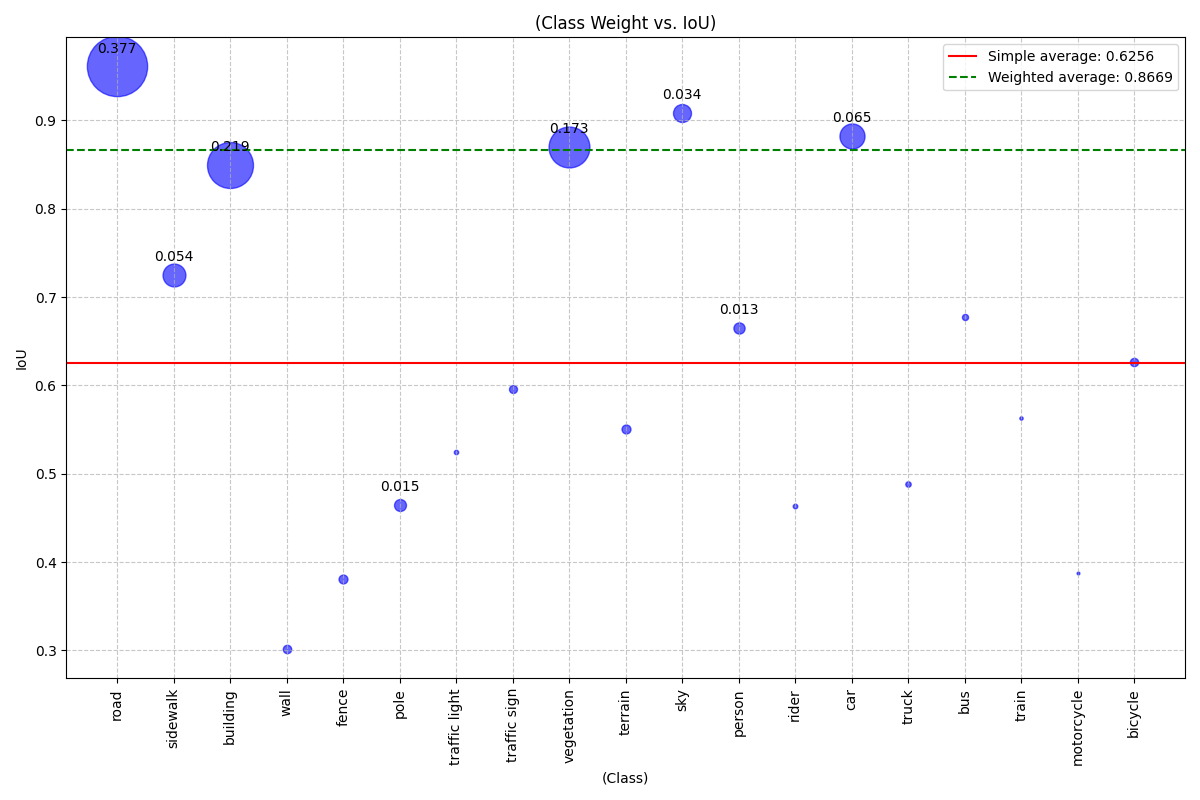
\includegraphics[width=0.8\textwidth]{outputs/deeplabv3plus_test_results/class_weight_vs_iou.png}
    \caption{Correlation between class weights and IoU scores, showing the relationship between class frequency and segmentation performance}
    \label{fig:class_weight_vs_iou}
\end{figure}



\end{document}